% Fig 2.13 -- the jump of a discrete cdf at a mass point a (web-original
%              figure, no manuscript tikzpicture; redrawn 2026-08-02 to
%              replace the hand-written SVG, which carried two lines of
%              Chinese sitting on the dashed gridlines)
% The jump height equals p_X(a) = F_X(a) - F_X(a^-).
\documentclass[tikz,border=2pt]{standalone}
\usepackage{amsmath}
\usepackage{amssymb}
\usepackage{xcolor}
\usetikzlibrary{arrows.meta}
\newcommand{\sssig}{\scriptscriptstyle}

\definecolor{journalink}{HTML}{1F1C18}
\definecolor{journalmuted}{HTML}{8A7F72}
\definecolor{journalaccent}{HTML}{9C2D2D}

\begin{document}
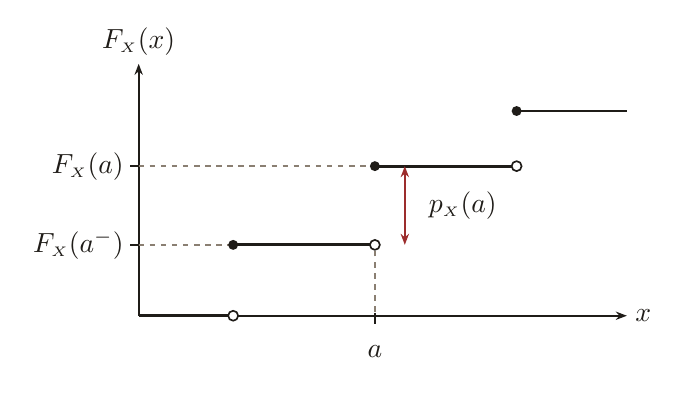
\begin{tikzpicture}[
  x=1cm,
  y=1cm,
  every node/.style={font=\normalsize, journalink},
  axis/.style={journalink, line width=0.8pt, -{Stealth[length=4pt]}},
  tick/.style={journalink, line width=0.8pt},
  stepline/.style={journalink, line width=1.0pt},
  guide/.style={journalmuted, line width=0.5pt, dash pattern=on 2pt off 2pt},
  jump/.style={journalaccent, line width=0.8pt,
               {Stealth[length=4pt]}-{Stealth[length=4pt]}},
  solidpt/.style={circle, fill=journalink, inner sep=0pt, minimum size=3.6pt},
  openpt/.style={circle, draw=journalink, line width=0.6pt, fill=white,
                 inner sep=0pt, minimum size=3.6pt}
]
  % ---- axes ----
  \draw[axis] (0,0) -- (6.2,0);
  \draw[axis] (0,0) -- (0,3.2);

  % ---- the mass point a on the x axis ----
  \draw[tick] (3,0.035) -- (3,-0.106);
  \node[anchor=north] at (3,-0.25) {$a$};

  % ---- y ticks at the two levels the jump runs between ----
  \draw[tick] (0.035,0.9) -- (-0.106,0.9)
    node[anchor=east, inner sep=2pt] {$F_{\sssig X}(a^{-})$};
  \draw[tick] (0.035,1.9) -- (-0.106,1.9)
    node[anchor=east, inner sep=2pt] {$F_{\sssig X}(a)$};

  % ---- guides (each stops at the endpoint it belongs to) ----
  \draw[guide] (0,0.9) -- (1.2,0.9);
  \draw[guide] (0,1.9) -- (3,1.9);
  \draw[guide] (3,0.05) -- (3,0.9);

  % ---- step segments ----
  \draw[stepline] (0,0)     -- (1.2,0);
  \draw[stepline] (1.2,0.9) -- (3,0.9);
  \draw[stepline] (3,1.9)   -- (4.8,1.9);
  \draw[stepline] (4.8,2.6) -- (6.2,2.6);

  % ---- jump height at a ----
  \draw[jump] (3.38,0.9) -- (3.38,1.9);
  \node[anchor=west] at (3.56,1.40) {$p_{\sssig X}(a)$};

  % ---- endpoints (drawn last, on top of the segments) ----
  \node[openpt]  at (1.2,0)   {};
  \node[solidpt] at (1.2,0.9) {};
  \node[openpt]  at (3,0.9)   {};
  \node[solidpt] at (3,1.9)   {};
  \node[openpt]  at (4.8,1.9) {};
  \node[solidpt] at (4.8,2.6) {};

  % ---- axis labels ----
  \node[anchor=west, inner sep=0pt] at (6.3,0) {$x$};
  \node[anchor=south, inner sep=0pt] at (0,3.3) {$F_{\sssig X}(x)$};
\end{tikzpicture}
\end{document}
